\documentclass[10pt]{article}
\usepackage[letterpaper,landscape,margin=0.65in]{geometry}
\usepackage{graphicx}
\usepackage[T1]{fontenc}
\usepackage{hyperref}
\hypersetup{pdftitle={Canonical GF(2^17) Frobenius and BINSTD factors}}
\setlength{\parindent}{0pt}
\setlength{\parskip}{0.48em}
\title{Canonical GF($2^{17}$) Frobenius and BINSTD factors}
\author{Validation audit, 22 October 2026}
\date{}
\begin{document}
\maketitle
\vspace{-2em}

\textbf{Frozen source.} The BINSTD n=17 dimension files record
bitmask factors 3, 313 and 471 of $X^{17}-1$ over $\mathbf F_2$.
Earlier Lean theorems bind those exact coefficients, prove their
product is $X^{17}+1$ and prove both degree-eight factors irreducible.

\textbf{New theorem.} For the canonical Mathlib field
$\mathrm{GF}(2^{17})$, the $\mathbf F_2$-linear Frobenius $x\mapsto x^2$
has order 17 and minimal polynomial equal to the archived three-factor
product. The proof instantiates Mathlib's finite-field Frobenius
theorems and rewrites $X^{17}-1=X^{17}+1$ in characteristic two.
The formal task targets both identities. Its verification receipt
reports a passing full build, standard axioms only across 630 audited
theorems, and a passing target audit under Lean 4.35.0-rc1.
Independent semantic review remains pending.

\textbf{Boundary.} The archived polynomial-basis runner uses
$t^{17}+t^3+1$. Its concrete field, Frobenius implementation and
subspace constructor are not identified with this canonical model in
Lean. Exhaustive invariant-subspace classification remains open.
No empirical yield, performance or security claim follows.

\newpage
\begin{center}
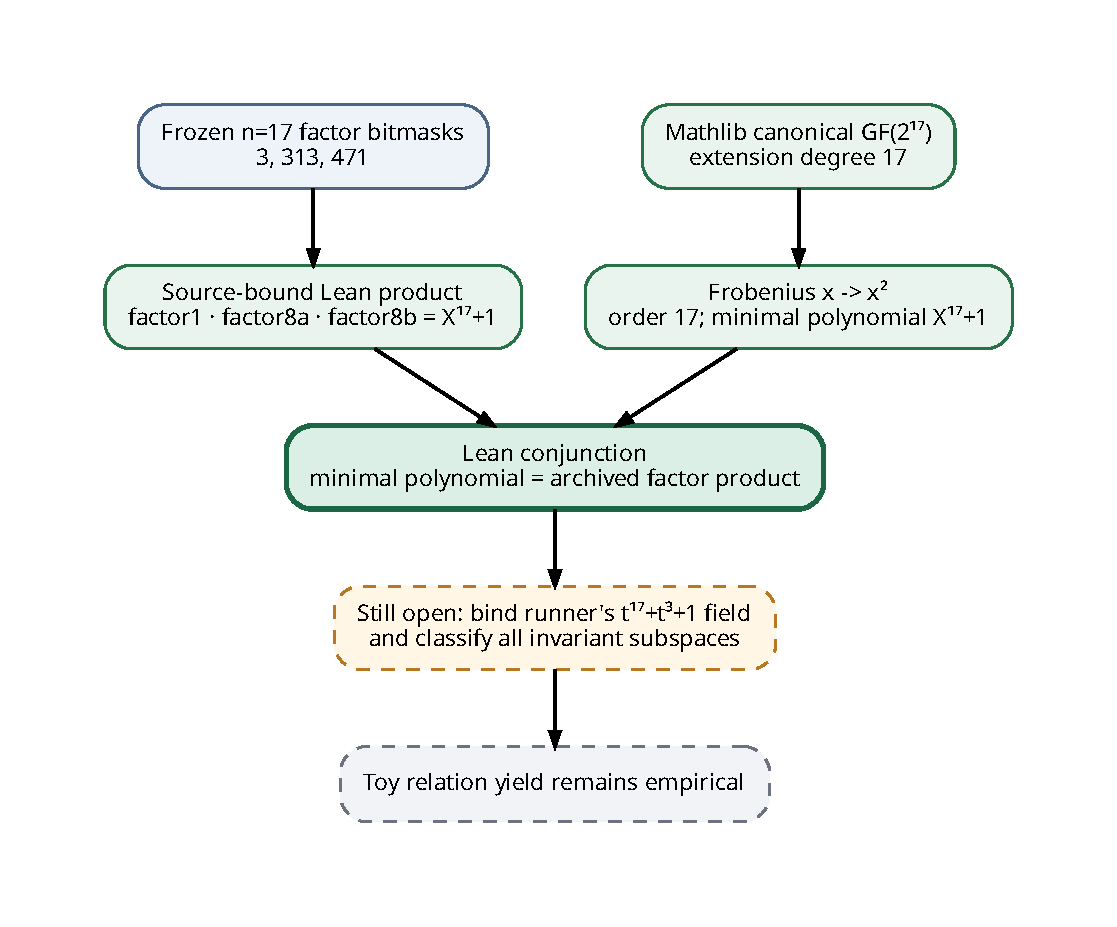
\includegraphics[width=\textwidth,height=0.82\textheight,keepaspectratio]{canonical-frobenius-figure.pdf}
\end{center}
\end{document}
